%%%%%%%%%%%%%%%%%%%%%%%%%%%%%%%%%%%%%%%%%%%%%%%%%%%%%%%%%%%%%%%%%%%%%%%%%
%
% LaTeX-Vorlage fuer die Gestaltung der Ausarbeitung zu einem Seminar
%
% Basierend auf einer Vorlage von Joerg Willmann vom 06.06.2002
% Ueberarbeitet von Clemens Juergens am 12.06.2002
%
%%%%%%%%%%%%%%%%%%%%%%%%%%%%%%%%%%%%%%%%%%%%%%%%%%%%%%%%%%%%%%%%%%%%%%%%%


\documentclass{seminar}
%\usepackage[applemac]{inputenc}
\usepackage[T1]{fontenc}
\usepackage[latin1]{inputenc}
\usepackage[english]{babel}
\usepackage{graphicx}
%\usepackage{url}
\usepackage[round]{natbib}
\usepackage{algorithm2e}
\usepackage{amsmath}
\usepackage{subcaption}




\begin{document}
	\renewcommand\toptitle{Seminar: ,,Current Topics in Deep Neural Networks``}
	\title{Neural Style Transfer}
	\author{Stefan Wezel}
	\maketitle
	
	
	\addvspace{0.5cm}
	\emph{\bfseries{Abstract:}}
	\emph{Introduced by \cite{gatys2015neural}, the field of neural style transfer (NST) has not only evolved rapidly but also allowed for insights into the processes inside neural networks as well as into human perception. Various methods, ranging from image-based to model-based approaches have been introduced to alleviate the weaknesses of the original formulation. Here, we recapture the idea behind \cite{gatys2015neural}'s algorithm and give an overview of methods, used in the current field of neural style transfer.}
	
	
	\tableofcontents
	\newpage
	
	\section{Introduction}
	Art has played an important role in human culture throughout most of its history [\cite{carroll2004art}]. Despite this, little is known about what the deciding neurological and psychological factors are for making us perceive something as aesthetic.
	In the past, the relationship between neurological science, psychology, and artificial intelligence has proven to be reciprocally beneficial. Especially the field of machine learning has yielded astonishing results, partially inspired by neurological foundations.
	On computer vision tasks, Convolutional Neural Nets have already outperformed humans, thus giving the impression that they may almost rival the perceptive prowess of the human visual cortex [\cite{geirhos2017comparing}].\\
	However, in Style Transfer, traditionally a subfield of non-photorealistic rendering, Neural Networks have yet to prove their capacity.
	\cite{gatys2015neural}'s work shows that they can be used to transfer arbitrary styles to any given content image. Besides the visually astonishing results, their work also gives insights into the creation and perception of artistic images.
	
	
	
	\section{Non-neural Style Transfer}
	Before Neural Networks were applied to Style Transfer, a popular approach to the problem existed in image-based artistic rendering [\cite{kyprianidis2012state}]. This area of research can be subdivided into multiple directions. \textbf{Linear Transformations}, i.e. Filters designed for image processing are used to create stylized images by \cite{winnemoller2006real} and \cite{tomasi1998bilateral} among others.\\ 
	Another popular approach, \textbf{Stroke-Based Rendering} typically starts with a photograph on which then strokes are placed iteratively in order to mimic a certain style. The placement of the strokes is optimized according to a given objective function which is some quantity that measures how similar the synthetic painting is to a specified image [\cite{hertzmann2003survey}]. Another technique is \textbf{Region-based Rendering} where an image is segmented into different regions. This enables a rendering algorithm to be sensitive to each region's specific content [\cite{kolliopoulos2005image}]. Both these approaches do lack the ability to incorporate any arbitrary style. Therefore, \cite{hertzmann2001image} proposes to learn a transformation from source to target image in a supervised fashion with the \textbf{Example-Based Rendering} technique of Image Analogies. This, however, requires training data which may not be available.\\
	While not having been designed for the goal of creating an artistic image, important contributions to style transfer research also come from \textbf{Texture Synthesis}. 
	Early work there focused on pixel measurements [\cite{julesz1962visual}].
	Later, filter responses played an important role in the work of \cite{heeger1995pyramid} and \cite{portilla2000parametric}. The use of summary statistics in Texture Synthesis can be viewed as a precursor to the neural style transfer algorithm proposed by \cite{gatys2015neural}. There, however, not the statistics of an image, but rather the statistics of the latent representation of an image are used for measuring similarity in style.\\
	Rather than using Descriptive Statistics, another branch of research exploits Markov Random Fields (MRF) in a \textbf{non-parametric modeling} approach to rendering stylized images. An MRF assumes that each pixel is characterized solely by the pixels in its spatial neighborhood [\cite{jing2019neural}].
	\cite{efros1999texture} find pixels in the texture image by finding pixels whose neighborhoods resemble each other and then replace them in the source image.\\
	The topic of neural style transfer can also be linked to \textbf{Image Reconstruction} where, rather than encoding images into latent representation, the goal is to create an image from given information. An approach, proposed by \cite{mahendran2015understanding} is able to generate images by optimizing latent representations. Given random noise, the algorithm iteratively optimizes the image up to a point where its latent representation matches that of those, generated by a convolutional net.
	This is computationally expensive because a new training process is required for every image. In order to generate images faster, \cite{dosovitskiy2016generating} propose to train a generative model to produce an image. Then, after a training stage, images can be computed in real-time, thus shifting the computational effort.
	
	
	
	
	\section{Original Algorithm of Neural Style Transfer}
	Using summarizing statistics from the feature representation of CNNs, \cite{gatys2015neural} propose an image-based approach to Style Transfer. %In their algorithm, a given image is optimized to match two source images, one is responsible for the content and the other one for the style of the image to optimize.
	\subsection{Setting}
	Given two images, one responsible for the content, and one for style, the goal of neural style transfer is to create a stylized image that matches the content images content and the style images style. The stylized image is iteratively optimized according to two loss terms.
	
	\subsection{VGG-Net}
	Convolutional Neural Networks have proven to represent features of input images efficiently once trained for a task like image classification. An architecture that became popular after winning the ILSVRC localization task in 2014 is the VGG-net [\cite{ILSVRC15}]. The VGG-net architecture (\ref{fig:vgg}) is characterized by stacking multiple convolutional layers, following a pooling operation. This is repeated multiple times up to one or more fully connected layers, which can serve as task-specific head \cite{simonyan2014very}.\\
	The latent representations from different convolutional layers are extracted by \cite{gatys2015neural} and serve as the basis for obtaining summarizing statistics.
	These statistics are used to transform the input image.
	
	%TODO find actual source of this image or draw yourself
	\begin{figure} %TODO maybe highlight layers which are used
		\centering
		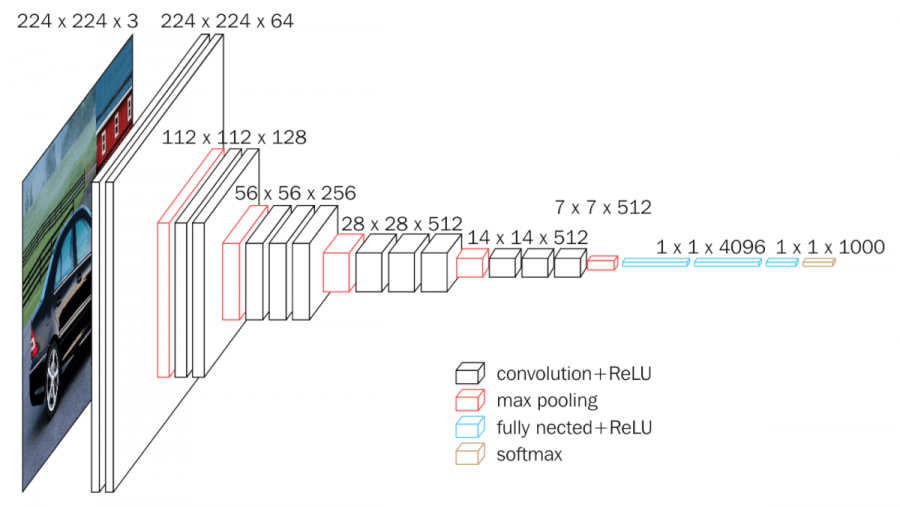
\includegraphics[scale=0.37]{vgg16.png}
		\caption{Architecture of the VGG net introduced by \cite{simonyan2014very}. \cite{gatys2015neural} extract feature representations from different convolutional layers of such a model. The diagram is taken from \cite{loukadakis2018accelerating}.}
		\label{fig:vgg}
	\end{figure}
	
	\subsection{Algorithm}
	The algorithm starts by extracting a content representation from the content image and style representation of the style image using the VGG-net. From the image, we want to optimize, we extract content as well as style. Then, the distance between the style representations and the content representations is measured. Each distance is a respective loss which gives us two quantities we can minimize. These two loss terms, style loss, and content loss are each multiplied with a small scalar and then added up, giving us our final loss term. Then, the gradient of the loss function for the current state of the input image is computed and backpropagated. However, only the input image is adjusted according to the gradient and none of the parameters of the VGG-net.
	
	
	\subsection{Content Representation and Loss}
	A convolutional layer $l$ with $n_l$ filters returns $n_l$ feature maps which mark the positions of where each respective feature occurred. The height and width of these feature maps are determined by the input and stride used [\cite{lecun1999object}]. To extract content information, \cite{gatys2015neural} propose to gather all feature maps of a layer in a feature Matrix $F_l\in\mathcal{R}^{n_l \times m_l}$ where $m_l$ equals the height times the width of the layers feature maps. Each feature map is vectorized and transposed, resulting in a feature vector which then becomes a column of the feature matrix. The level of abstraction of features in $F_l$ is sensitive to the choice of $l$. \cite{gatys2015neural} propose to use a layer that captures the shapes and layout of the input image rather than finer features such as texture information.\\
	To measure the difference between an input image $x$ and content image $p$, \cite{gatys2015neural} propose to generate respective feature matrices $F^l$ and $P^l$ and measure mean square distance between these:\\
	\begin{align}
	\mathcal{L}_{content}(p, x, l) = \frac{1}{2}\sum_{ij}(F^l_{ij} - P^l_{ij})^2
	\end{align}
	
	
	
	\subsection{Style Representation and Loss}
	The style of an image is invariant to the spatial arrangement of its features. Thus, the style representation should be spatially invariant as well. Since feature maps contain spatial information and therefore cannot be used to represent style, \cite{gatys2015neural} propose to measure their co-occurrence in an image. For this purpose, they make use of the Gram matrix.\\
	The Gram matrix of a set of vectors contains the inner product of all combinations of vectors from the set. In the case of neural style transfer, the set of vectors is the set of vectorized feature maps of a layer $l$.
	By calculating the inner product of each of the feature vectors, all spatial information is removed. Remaining is the information about how often the features appear in the same position. This gives us a spatially invariant representation of style by capturing what features correlate rather than where a feature appears.
	\begin{align}
	G^l_{ij} = \sum_{k} F^l_{ik}F^l_{jk}
	\end{align}
	\cite{gatys2015neural} found that using multiple layers for the style representation produces visually more appealing results. So in order to measure similarity in style of input image $x$ and style image $a$, the respective Gram matrices $G^l$ and $A^l$ are computed.
	The loss term is
	\begin{align*}
	L_{style}(a,x) = \sum^L_{l=0}w_l E_l
	\end{align*}
	where 
	\begin{align*}
	E_l = \frac{1}{4n^2_lm^2_l}\sum_{ij}(G^l_{ij}-A^l_{ij})^2
	\end{align*}
	and $w_l$ weights each layers contribution to the style loss.
	
	\subsection{Total Loss and Optimization}
	The total loss term is composed of the style loss and the content loss, each weighted by a factor.
	\begin{align*}
	\mathcal{L}_{total}(p, a, x) = \alpha \mathcal{L}_{content}(p,x) + \beta \mathcal{L}_{style}(a,x)
	\end{align*}
	where $\alpha$ and $\beta$ are hyperparameters that determine the style/content trade-off.\\
	In order to compute gradients that can be backpropagated to the input image, style, and content loss need to be derived according to the layer's activation. For content loss, we can compute the derivative with
	\begin{align*}
	\frac{\partial \mathcal{L}_{content}}{\partial F^l_{ij}} = 
	\begin{cases}
	(F^l-P^l)_{ij} & \text{if}\ F^l_{ij} > 0 \\
	0 & \text{if} F^l_{ij} <0
	\end{cases}
	\end{align*}
	where as style loss can be differentiated as follows:
	\begin{align*}
	\frac{\partial E_l}{\partial F^l_{ij}} =
	\frac{1}{n_l^2m_l^2}((F^l)^T (G^l-A^l))_{ij} & \text{ if}\ F^l_{ij} > 0 \\
	0 & \text{ if} F^l_{ij} < 0
	\end{align*}
	
	\section{Derivations and Alternative Approaches}
	Despite the field of neural style transfer being rather young, many alternatives, derivations, and improvements to \cite{gatys2015neural} algorithm have been proposed. Generally, we can differ between two approaches. \text{Image-based approaches} iteratively optimize an input image to match the source image's content and style. This, however, requires a new training process for every new image. The many resulting backward passes are computationally expensive. Instead of adjusting an input image, \textbf{Model-based approaches} optimize a generative model that creates stylized images. Thus shifting the computational cost towards the training stage and making a real-time generation of stylized images possible. In only a few years, many ideas for both approaches have been proposed. In the following section, we will have a look at some of those ideas and briefly discuss their benefits and drawbacks.
	
	\subsection{Image-Based}
	\cite{simonyan2013deep}'s algorithm for interpreting features learned by a convolutional neural net can be viewed as a precursor to neural style transfer. They optimize the input image to maximally activate a specified subset, i.e. a layer, feature map, or single neuron of a convolutional neural net.
	The previously discussed algorithm of \cite{gatys2015neural} then opened the field of neural style transfer with their image-based approach. The proposed optimization process, however, suffers from instability during training which often results in noisy stylized images. 
	\cite{risser2017stable} found that this is due to feature maps with different means and variances can still have a similar Gram matrix. To alleviate this, they calculate the distribution of feature activations of style image and input image representations and then compare the difference of the resulting distribution's histogram. This difference is then added as a third loss term.
	Besides the presented approaches, there exist many more and this is only a small subset of ideas developed in the last few years.
	
	\subsection{Model-Based}
	The field of model-based approaches can be subdivided into three groups which differ in their setting. In the \textbf{Single-style-per-model} setting, a generative model is trained to match one specific style. This could for example be achieved by creating a large dataset of input content and stylized target images with an image-based Algorithm and then train the generative model using on this dataset. Most of these approaches only differ in the network architecture used for the generative model [\cite{jing2019neural}]. One such example, proposed by \cite{johnson2016perceptual} is depicted in \ref{fig:johnson}.\\
	A more challenging setting is \textbf{Multiple-style-per-model} where one model is ideally able to create images in one of multiple pre-defined styles. A common idea for this is, to try and make only a subset of parameters responsible for one style and ideally be able to share parameters. One such approach was proposed by \cite{chen2017stylebank}, whose model learns representations for style and content individually. They use an encoder to learn content representations, a 'StyleBank' layer which contains specific filters for each style that can be chosen and a decoder that produces the stylized image, using the chosen filters from the 'StyleBank' layer. Images created by this approach are depicted in \ref{fig:stylebank}.\\
	The category of model-based which matches the flexibility of image-based approaches the closest is \textbf{Arbitrary-style-per-model}. This setting is difficult and various, often quite different approaches exist. \cite{chen2016fast} find for each patch of feature representations from the content image the most similar patch in the representation of the style image and then replace it. The idea is to find representations that are responsible for style in the content image and then swap them with style information from the style image. Results from \cite{chen2016fast} are shown in \ref{fig:chen}.
	
	
	
	
	\begin{figure}[h]
		\centering
		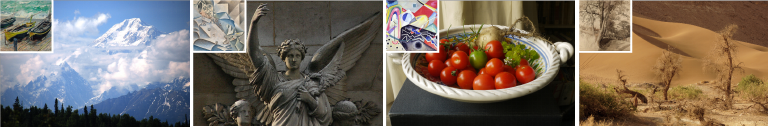
\includegraphics[width=\textwidth]{nst_source.png}
		\caption{Content and style images.}\label{fig:source}
		%\bigbreak
		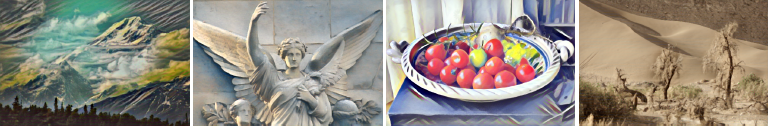
\includegraphics[width=\textwidth]{nst_johnson.png}
		\caption{\cite{johnson2016perceptual}}\label{fig:johnson}
		%\bigbreak
		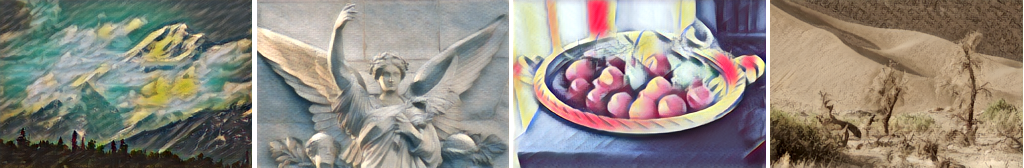
\includegraphics[width=\textwidth]{nst_stylebank.png}
		\caption{\cite{chen2017stylebank}}\label{fig:stylebank}
		%\bigbreak
		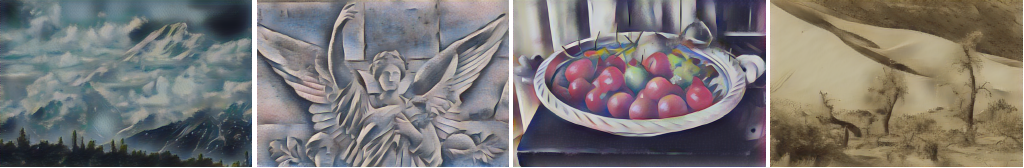
\includegraphics[width=\textwidth]{nst_chen.png}
		\caption{\cite{chen2016fast}}\label{fig:chen}
		\bigbreak
		%\caption{Various model based approaches compared on different content and style images.}
	\end{figure}
	
	\section{Challenges and Future Directions}
	Despite the rapid progress of the only recently introduced field of neural style transfer, there are still many open challenges that have yet to be overcome.
	
	\subsection{Evaluation}
	One key challenge is the evaluation of different models and algorithms. Since the result of neural style transfer is inherently subjective, coming up with a unified and agreed upon evaluation protocol is a difficult task. In recent publications, researchers often evaluated their novel techniques by showing side-by-side comparisons of their work next to existing techniques. \cite{jing2019neural} propose to conduct a study with eight individuals that rate the results of different NST approaches. However, their ratings varied a lot, despite most of their subjects were of the same age and background. Also, such an approach is expensive as well as difficult to organize and replicate.\\
	\cite{jing2019neural} also propose to involve professionals, such as artists and designers into an evaluation process to measure performance according to agreed-upon aesthetic principles.\\
	They also suggest that the NST research community would benefit from a benchmark dataset. Such benchmarks datasets have in the past caused large leaps in different areas of machine learning. A solution for this could be to use benchmark datasets from related areas, such as Non-photorealistic rendering. Meanwhile, NST is not only limited to image data, but is now also applied in video and 3D data [\cite{huang2017real}, \cite{kato2018neural}], so it would be necessary to agree on benchmark datasets for those categories as well.
	
	
	\subsection{Interpretability}
	Another important issue is the interpretability of models and algorithms used for neural style transfer. All of the covered approaches use black-box models like convolutional neural networks. Generally, it is not trivial to understand what features they learn and use for producing an output. In the case of an undesired or unsatisfying result, it is then difficult to see how changes made to the model or training process would affect the outcome. This then often results in a trial-and-error process.\\
	Using models that learn \textbf{disentangled representations} could to some extend alleviate this problem. The definition of disentanglement in the context of machine learning is not agreed upon and the subject of debate [\cite{higgins2018towards}]. Usually, it is assumed for a model that learns disentangled representation to encode the independent generating factors of data as separate dimensions in a latent representation thus creating interpretable representations that would ideally resemble real-world observable variables. This would not only make neural style transfer more interpretable but also more controllable and therefore more applicable because it could allow for tools, where different aspects of a certain style, such as stroke direction, brush size, lighting among many others could be controlled by a user.\\
	However, the field of disentangled representation learning is challenging in itself.
	The mere possibility of unsupervised learning of disentangled representations is debated [\cite{locatello2018challenging}]. On the other side, learning disentangled representation in a supervised fashion may be unreasonable since it would require large datasets that would need to be variant to the many different aspects of a certain style.
	
	
	
	
	
	\section{Applications}
	To be applied in a broader set of real-world settings, neural style transfer has yet to overcome many of the discussed challenges.\\
	An area where NST is already applied is \textbf{social media}. Apps like Prisma [\cite{prisma}] have made NST a popular way to create and share stylized photographs. By making NST available to a large number of users, \cite{jing2019neural} hypothesis that NST research could use the perception of different stylized images in order to move towards a more quantitative evaluation. Mobile devices play a large role in social media but have only limited computational resources. For more widespread use of NST on such edge devices, the developing community would have to come up with computationally less expensive methods.\\
	An even more challenging setting for applied NST is that of \textbf{User-assisted Creation Tools}. For example, design tools, that help users integrate a certain style into their work could be able to speed up creation processes.\\
	Such tools could be used in \textbf{Production of Entertainment Products}. Use of Computer Generated Imagery (CGI) has increased ever since its inception [\cite{tucker2007movies}]. Integrating certain styles into CGI is an elaborate process that requires programming shaders and the work of artists [\cite{apodaca2000advanced}]. Tools that could render given images in a specified style could alleviate some of the technical difficulties of this process and speed up production as well as make it more flexible since ideally styles could be manipulated after animating sequences and would be invariant to the underlying imagery.\\
	Besides those discussed, it is very likely that there are many more approaches to which some of them may only emerge, once the field of NST itself has progressed even further.
	
	
	
	\section{Conclusion}
	The field of neural style transfer is, despite its very recent emergence interesting and fast developing. It motivates us to further engage with the processes inside deep neural networks. \cite{gatys2015neural} hypothesize that it can even help us understand the underlying principles of what makes something aesthetically appealing to humans. That Convolutional Neural Networks excel in such an area further proves their power and versatility. It also shows that meaningful and good representations can be useful for downstream tasks, even ones previously not thought about. However, many open challenges remain as the field of neural style transfer matures.
	
	
	
	
	
	\newpage
	
	% Variante mit seperatem Bibtex-File
	
	\bibliographystyle{natbib}
	\bibliography{seminarRefs}
	
	
	% Variante zum manuellen Eintragen der Referenzen
	%\begin{thebibliography}{01}
	%\bibitem[Hunt98]{Hunt98}
	%C. Hunt, TCP/IP Network Administration, O'Reilly 1998.
	%\bibitem[Schnei94]{Schnei94}
	%Dr. G. Schneider, Internet: Werkzeuge und Dienste, Springer-Verlag
	%Berlin Heidelberg 1994.
	%\end{thebibliography}
\end{document}



